\documentclass{standalone}
\usepackage{tikz}
\usetikzlibrary{patterns, positioning}


\begin{document}
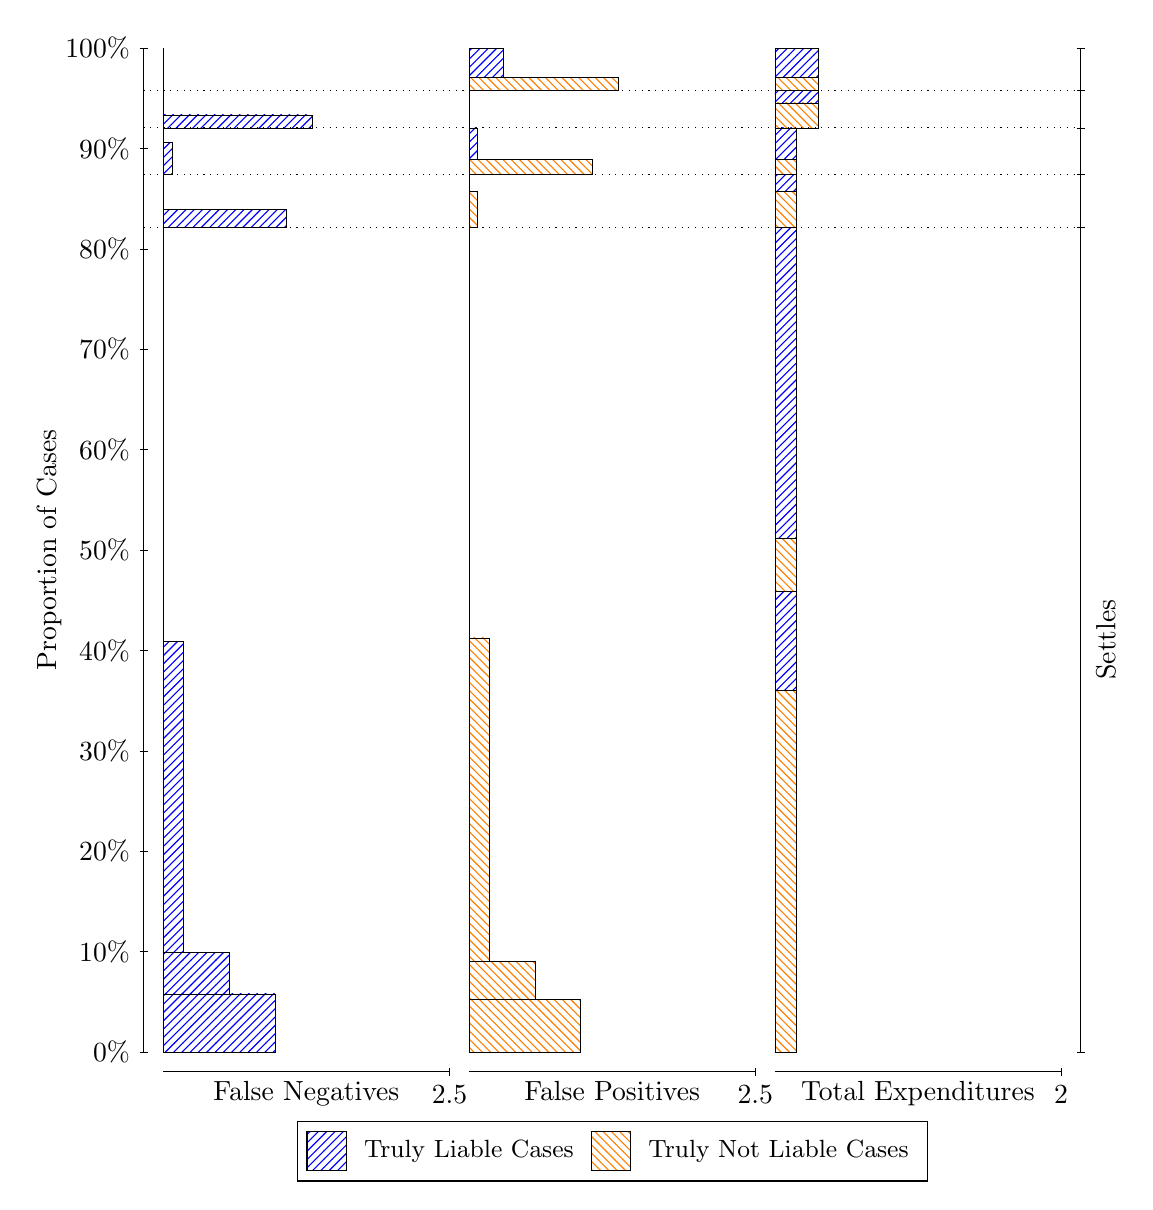
\begin{tikzpicture}
\draw[black, very thin] (1.5,1.75) -- (1.5,14.5);
\node[rotate=90, text=black, anchor=center] at (0.3, 8.125) {Proportion of Cases};
\draw[black, very thin] (1.45,1.75) -- (1.55,1.75);
\node[text=black, anchor=east] at (1.45, 1.75) {0\%};
\draw[black, very thin] (1.45,3.025) -- (1.55,3.025);
\node[text=black, anchor=east] at (1.45, 3.025) {10\%};
\draw[black, very thin] (1.45,4.3) -- (1.55,4.3);
\node[text=black, anchor=east] at (1.45, 4.3) {20\%};
\draw[black, very thin] (1.45,5.575) -- (1.55,5.575);
\node[text=black, anchor=east] at (1.45, 5.575) {30\%};
\draw[black, very thin] (1.45,6.85) -- (1.55,6.85);
\node[text=black, anchor=east] at (1.45, 6.85) {40\%};
\draw[black, very thin] (1.45,8.125) -- (1.55,8.125);
\node[text=black, anchor=east] at (1.45, 8.125) {50\%};
\draw[black, very thin] (1.45,9.4) -- (1.55,9.4);
\node[text=black, anchor=east] at (1.45, 9.4) {60\%};
\draw[black, very thin] (1.45,10.675) -- (1.55,10.675);
\node[text=black, anchor=east] at (1.45, 10.675) {70\%};
\draw[black, very thin] (1.45,11.95) -- (1.55,11.95);
\node[text=black, anchor=east] at (1.45, 11.95) {80\%};
\draw[black, very thin] (1.45,13.225) -- (1.55,13.225);
\node[text=black, anchor=east] at (1.45, 13.225) {90\%};
\draw[black, very thin] (1.45,14.5) -- (1.55,14.5);
\node[text=black, anchor=east] at (1.45, 14.5) {100\%};

\draw[black, very thin] (13.4,1.75) -- (13.4,14.5);
\draw[black, very thin] (13.35,1.75) -- (13.45,1.75);
\node[anchor=west] at (13.35, 1.75) {};
\draw[black, very thin] (13.35,12.226) -- (13.45,12.226);
\node[anchor=west] at (13.35, 12.226) {};
\draw[black, very thin] (13.35,12.895) -- (13.45,12.895);
\node[anchor=west] at (13.35, 12.895) {};
\draw[black, very thin] (13.35,13.487) -- (13.45,13.487);
\node[anchor=west] at (13.35, 13.487) {};
\draw[black, very thin] (13.35,13.966) -- (13.45,13.966);
\node[anchor=west] at (13.35, 13.966) {};
\draw[black, very thin] (13.35,14.5) -- (13.45,14.5);
\node[anchor=west] at (13.35, 14.5) {};

\draw[black, very thin, pattern color=blue, pattern=north east lines] (1.75,1.75) rectangle (3.167,2.4878);
\draw[black, very thin, pattern color=blue, pattern=north east lines] (1.75,2.4878) rectangle (2.5857,3.0109);
\draw[black, very thin, pattern color=blue, pattern=north east lines] (1.75,3.0109) rectangle (2.0043,6.968);
\draw[black, very thin, pattern color=orange, pattern=north west lines] (1.75,6.968) rectangle (1.75,12.226);
\draw[black, very thin, pattern color=blue, pattern=north east lines] (1.75,12.226) rectangle (3.3123,12.446);
\draw[black, very thin, pattern color=orange, pattern=north west lines] (1.75,12.446) rectangle (1.75,12.895);
\draw[black, very thin, pattern color=blue, pattern=north east lines] (1.75,12.895) rectangle (1.859,13.298);
\draw[black, very thin, pattern color=orange, pattern=north west lines] (1.75,13.298) rectangle (1.75,13.487);
\draw[black, very thin, pattern color=blue, pattern=north east lines] (1.75,13.487) rectangle (3.6393,13.65);
\draw[black, very thin, pattern color=orange, pattern=north west lines] (1.75,13.65) rectangle (1.75,13.966);
\draw[black, very thin, pattern color=orange, pattern=north west lines] (1.75,13.966) rectangle (1.75,14.129);
\draw[black, very thin, pattern color=blue, pattern=north east lines] (1.75,14.129) rectangle (1.75,14.5);
\draw[black, very thin, pattern color=orange, pattern=north west lines] (5.6333,1.75) rectangle (7.0503,2.4153);
\draw[black, very thin, pattern color=orange, pattern=north west lines] (5.6333,2.4153) rectangle (6.469,2.899);
\draw[black, very thin, pattern color=orange, pattern=north west lines] (5.6333,2.899) rectangle (5.8877,7.0076);
\draw[black, very thin, pattern color=blue, pattern=north east lines] (5.6333,7.0076) rectangle (5.6333,12.226);
\draw[black, very thin, pattern color=orange, pattern=north west lines] (5.6333,12.226) rectangle (5.7423,12.675);
\draw[black, very thin, pattern color=blue, pattern=north east lines] (5.6333,12.675) rectangle (5.6333,12.895);
\draw[black, very thin, pattern color=orange, pattern=north west lines] (5.6333,12.895) rectangle (7.1957,13.084);
\draw[black, very thin, pattern color=blue, pattern=north east lines] (5.6333,13.084) rectangle (5.7423,13.487);
\draw[black, very thin, pattern color=orange, pattern=north west lines] (5.6333,13.487) rectangle (5.6333,13.803);
\draw[black, very thin, pattern color=blue, pattern=north east lines] (5.6333,13.803) rectangle (5.6333,13.966);
\draw[black, very thin, pattern color=orange, pattern=north west lines] (5.6333,13.966) rectangle (7.5227,14.129);
\draw[black, very thin, pattern color=blue, pattern=north east lines] (5.6333,14.129) rectangle (6.0693,14.5);
\draw[black, very thin, pattern color=orange, pattern=north west lines] (9.5167,1.75) rectangle (9.7892,6.3423);
\draw[black, very thin, pattern color=blue, pattern=north east lines] (9.5167,6.3423) rectangle (9.7892,7.6032);
\draw[black, very thin, pattern color=orange, pattern=north west lines] (9.5167,7.6032) rectangle (9.7892,8.2685);
\draw[black, very thin, pattern color=blue, pattern=north east lines] (9.5167,8.2685) rectangle (9.7892,12.226);
\draw[black, very thin, pattern color=orange, pattern=north west lines] (9.5167,12.226) rectangle (9.7892,12.675);
\draw[black, very thin, pattern color=blue, pattern=north east lines] (9.5167,12.675) rectangle (9.7892,12.895);
\draw[black, very thin, pattern color=orange, pattern=north west lines] (9.5167,12.895) rectangle (9.7892,13.084);
\draw[black, very thin, pattern color=blue, pattern=north east lines] (9.5167,13.084) rectangle (9.7892,13.487);
\draw[black, very thin, pattern color=orange, pattern=north west lines] (9.5167,13.487) rectangle (10.062,13.803);
\draw[black, very thin, pattern color=blue, pattern=north east lines] (9.5167,13.803) rectangle (10.062,13.966);
\draw[black, very thin, pattern color=orange, pattern=north west lines] (9.5167,13.966) rectangle (10.062,14.129);
\draw[black, very thin, pattern color=blue, pattern=north east lines] (9.5167,14.129) rectangle (10.062,14.5);
\draw[black, dotted] (1.5,12.226) -- (13.4,12.226);
\draw[black, dotted] (1.5,12.895) -- (13.4,12.895);
\draw[black, dotted] (1.5,13.487) -- (13.4,13.487);
\draw[black, dotted] (1.5,13.966) -- (13.4,13.966);
\draw[black, very thin] (1.75,1.5) -- (5.3833,1.5);
\node[text=black, anchor=north] at (3.5667, 1.5) {False Negatives};
\draw[black, very thin] (5.3833,1.45) -- (5.3833,1.55);
\node[text=black, anchor=north] at (5.3833, 1.45) {2.5};

\draw[black, very thin] (5.6333,1.5) -- (9.2667,1.5);
\node[text=black, anchor=north] at (7.45, 1.5) {False Positives};
\draw[black, very thin] (9.2667,1.45) -- (9.2667,1.55);
\node[text=black, anchor=north] at (9.2667, 1.45) {2.5};

\draw[black, very thin] (9.5167,1.5) -- (13.15,1.5);
\node[text=black, anchor=north] at (11.333, 1.5) {Total Expenditures};
\draw[black, very thin] (13.15,1.45) -- (13.15,1.55);
\node[text=black, anchor=north] at (13.15, 1.45) {2};

\node[text=black, centered, rotate=90] at (13.72, 6.9878) {Settles};





\draw (7.449999999999999,1.5) node[draw=none] (baseCoordinate) {};
\begin{scope}[align=center]
        \matrix[scale=0.5, draw=black, below=0.5cm of baseCoordinate, nodes={draw}, column sep=0.1cm]{
            \node[rectangle, draw, minimum width=0.5cm, minimum height=0.5cm, pattern color=blue, pattern=north east lines] {}; &
            \node[draw=none, font=\small, text=black] (B) {Truly Liable Cases}; &
            \node[rectangle, draw, minimum width=0.5cm, minimum height=0.5cm, pattern color=orange, pattern=north west lines] {}; &
            \node[draw=none, font=\small, text=black] (B) {Truly Not Liable Cases}; \\
            };
\end{scope}

\end{tikzpicture}
\end{document}